\documentclass[12pt,a4paper]{article}
\usepackage[margin=21mm]{geometry}
\usepackage[T1]{fontenc}
\usepackage[scaled]{helvet}
\renewcommand{\familydefault}{\sfdefault}
\usepackage{microtype,xcolor,tikz,enumitem,fancyhdr,ragged2e}
\usepackage[hidelinks]{hyperref}
\definecolor{ink}{HTML}{1C2834}
\definecolor{muted}{HTML}{304E62}
\definecolor{light}{HTML}{EFF5FA}
\color{ink}
\setlength{\parindent}{0pt}
\setlength{\parskip}{7pt}
\linespread{1.05}
\pagestyle{fancy}\fancyhf{}
\fancyfoot[L]{\small Ground shakes\enspace|\enspace5 November 2026}
\fancyfoot[R]{\small\thepage\ of 2}
\renewcommand{\headrulewidth}{0pt}
\renewcommand{\footrulewidth}{0pt}
\newcommand{\heading}[1]{\par\vspace{6pt}{\large\bfseries #1}\par}
\newcommand{\finding}[2]{\textbf{#1}\ #2\par}
\newcommand{\records}{1,531}
\newcommand{\candidates}{1,516}
\newcommand{\early}{1,179}
\newcommand{\doubleRecords}{101}
\newcommand{\doubleTotal}{716}

\hypersetup{pdftitle={Ground shakes: what we measured and what we found},
 pdfsubject={Plain-language summary of saved ProtoDUNE-HD detector signals; historical PDS orientation checked}}
\begin{document}
\raggedright
\hyphenpenalty=10000
\exhyphenpenalty=10000
\emergencystretch=2em
{\LARGE\bfseries Ground shakes: what we found}\par
\textbf{We see a clear disturbance in the saved detector signals. We still do not know what causes it.}

``Ground shake'' is the name used for this disturbance. The records measure
electrical signals in the detector. They do not measure physical shaking.

\heading{The records we checked}
We reviewed \records{} saved records from seven ProtoDUNE-HD runs in July,
October and November 2024. An automatic check found \candidates{} records with
a large disturbance on both charge-readout panels.
These selected files cannot tell us how often this happens in normal operation.

The charge detector, or TPC, records signals on wires. The light-detector
system, or PDS, records signals through DAPHNE electronics. We compared their
signal sizes, times and positions. We also checked archived voltage and current records.

\heading{The checks and what they tell us}
\finding{Early pulses.}{We found sharp PDS pulses before the main disturbance in
\early{} of the \candidates{} selected records. Missing recording time prevents
us from saying whether every disturbance has an earlier pulse.}

\finding{Two pulses.}{In run 32731, \doubleRecords{} of \doubleTotal{} selected records
had at least two pulses between 300 and 100 microseconds before the main disturbance.
A microsecond is one millionth of a second. These are pulse candidates, not confirmed flashes of light.}

\finding{Electrical response.}{We used inputs reported as disconnected to predict
signals on connected inputs. They explained part of the response. This does not
separate all electrical interference from real light.}

\finding{Charge and light timing.}{We compared pulse times with nearby activity on
TPC wires. A delay pattern remained when we swapped PDS records between events.
We have not identified a unique charge--light match. A source repeating in the same place remains possible.}

\finding{Position and electronics.}{The slow activity before the main disturbance
was strongest in upper modules. Signals sharing an electronics group also tended
to match more closely during the main disturbance. Neither result locates the cause.}

\finding{Voltage and current.}{The checks found no clear relationship that held
across both November runs. These minute-scale records cannot show very fast voltage or current changes.}

\newpage
{\LARGE\bfseries Reading the detector map}\par
A channel is one recorded input. A module is a physical light-detector unit
with four readout channels. The modules sit in the charge-readout panels,
called APA1 and APA2. M means module.

\heading{Upper modules had the strongest slow activity}
\begin{center}
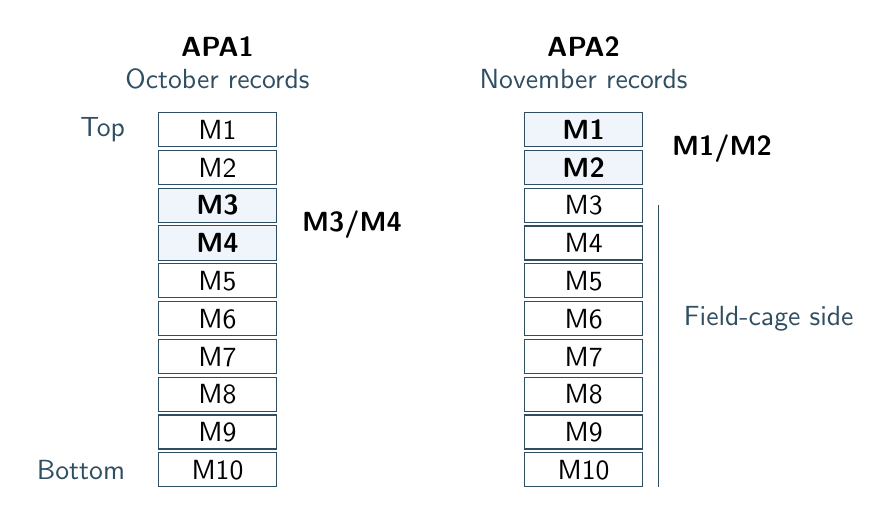
\begin{tikzpicture}[x=1cm,y=0.48cm,font=\normalsize]
  \node[font=\bfseries] at (1.35,1.2) {APA1};
  \node[font=\bfseries] at (6.0,1.2) {APA2};
  \node[text=muted] at (1.35,0.35) {October records};
  \node[text=muted] at (6.0,0.35) {November records};
  \foreach \m in {1,...,10} {
    \pgfmathsetmacro{\y}{-\m}
    \draw[muted] (0.6,\y-0.45) rectangle (2.1,\y+0.45);
    \draw[muted] (5.25,\y-0.45) rectangle (6.75,\y+0.45);
    \node at (1.35,\y) {M\m};
    \node at (6,\y) {M\m};
  }
  \foreach \m in {3,4} {
    \pgfmathsetmacro{\y}{-\m}
    \fill[light] (0.61,\y-0.44) rectangle (2.09,\y+0.44);
    \node[font=\bfseries] at (1.35,\y) {M\m};
  }
  \foreach \m in {1,2} {
    \pgfmathsetmacro{\y}{-\m}
    \fill[light] (5.26,\y-0.44) rectangle (6.74,\y+0.44);
    \node[font=\bfseries] at (6,\y) {M\m};
  }
  \node[anchor=east,text=muted] at (0.3,-1) {Top};
  \node[anchor=east,text=muted] at (0.3,-10) {Bottom};
  \node[anchor=west,align=left] at (2.3,-3.5) {\textbf{M3/M4}};
  \node[anchor=west,align=left] at (7,-1.5) {\textbf{M1/M2}};
  \draw[muted] (6.95,-3) -- (6.95,-10.45);
  \node[anchor=west,align=left,text=muted] at (7.15,-6) {Field-cage\ side};
\end{tikzpicture}
\end{center}
{\small Separate views in the source-map orientation; spacing is schematic. Bold rows mark the strongest
slow activity in 39 of 49 usable APA1 records and 1,210 of 1,224 APA2 records.
These are different runs, not simultaneous views of the same events.}

\heading{The channel orientation was checked}
We checked all 40 channel positions in each map against the historical source.
M1 is at the top; M10 is at the bottom. In the APA2 view, the field cage is on
the right. The field cage shapes the electric field inside the TPC. The top row reads \textbf{27, 25, 22, 20} from left to right.
Channel 20 is at the top-right corner.

The source photograph was mirrored to match this view. APA1 has a different
channel order. This is a check against the historical map, not a new survey
of the installed detector. We have not assigned beam or compass directions.

\heading{What we still need to learn}
We have not found one module that always starts first. Several modules often
start too close together to separate with the current timing. We need longer
recordings. We also need to measure each channel's own delay and use the wire
signals to work out where charge came from. These checks can help test where
the disturbance begins and whether light is involved.

{\small\color{muted}
\textbf{Sources.} A. Cervera, \href{https://edms.cern.ch/document/3493627/1}{EDMS 3493627 v1},
pp.\ 18, 20--21 (historical working presentation).
\href{../../../ground-shake-data/analysis/apa1-apa2-response-20261103/MODULES.txt}{Module measurements},
\href{../../../ground-shake-data/analysis/module-first-histogram-20261104/README.txt}{timing checks},
and \href{README.md}{full source notes} accompany this report.
}
\end{document}
